\begin{table}[t]
\centering
\caption{Anvil registration cost on the full TinyLlama workload. Gas and
new state are means per model. Setup and deployment are reported
separately in the repository.}
\label{tab:registration}
\begin{tabular}{lrrr}
\toprule
Design & Tx count & Gas/model & Bytes/model \\
\midrule
D1 & 2,317 & 571,877 & 746.7 \\
D2 & 2,317 & 614,533 & 792.4 \\
D3 ($k=1$) & 2,317 & 79,603 & 64.0 \\
D3 ($k=16$) & 145 & 4,989 & 4.0 \\
D3 ($k=128$) & 19 & 660 & 0.5 \\
\bottomrule

\end{tabular}
\end{table}

\begin{table}[t]
\centering
\caption{Median local timing and throughput on the full TinyLlama
workload. D1 has no separate policy measurement.}
\label{tab:timing}
\begin{tabular}{lrrr}
\toprule
Design & Policy (ms) & Verify (ms) & Audit (models/s) \\
\midrule
D1 & -- & 19.90 & 80.27 \\
D2 & 4.67 & 18.80 & 75.17 \\
D3 ($k=1$) & 0.95 & 4.98 & 192.14 \\
D3 ($k=16$) & 0.82 & 4.77 & 212.30 \\
D3 ($k=128$) & 0.73 & 4.59 & 209.43 \\
\bottomrule

\end{tabular}
\end{table}

Table~\ref{tab:registration} compares the same registration workload
across five configurations. D2 adds policy state and checks to the
direct registry. D3 stores one commitment and a compact batch record per
transaction. A larger batch spreads that transaction and state cost
across more models. The batch approach moves policy evaluation and the
record index to the attester. These results measure the on-chain costs
of the implemented designs under the stated trust assumptions.
New state per model is amortized across models in an anchored batch.

Table~\ref{tab:timing} reports the median policy and verification times
for the sampled records and the median throughput across the five audit
passes. D2 policy timing includes simulating the registration call.
D3 policy timing includes the OPA HTTP round trip. Verification timing
includes retrieving state through local RPC and checking the lineage
against the expected commitments.

\begin{figure*}[t]
\centering
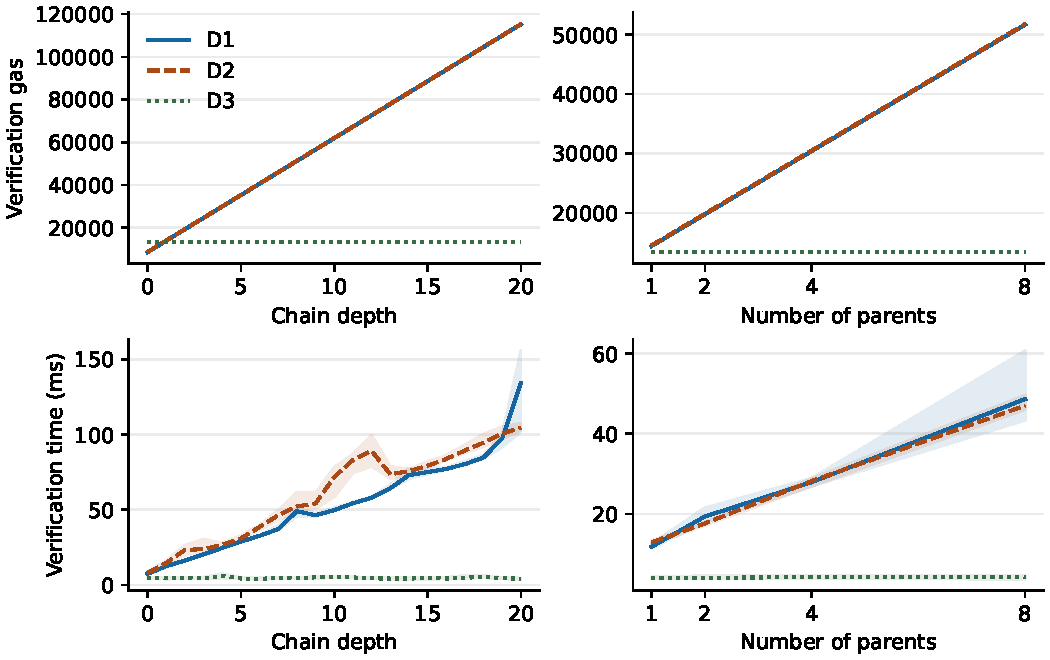
\includegraphics[width=0.94\textwidth]{synthetic_scaling.pdf}
\caption{Synthetic verification scaling on Anvil. D3 uses batches of
one model to hold proof size fixed. Shaded bands show the interquartile
range of wall-clock observations. D1 and D2 gas curves nearly overlap.}
\label{fig:scaling}
\end{figure*}

Figure~\ref{fig:scaling} separates chain depth from parent fan-in.
D1 and D2 walk additional records as either workload grows, increasing
gas and local verification time. D3 reconstructs the target commitment
off-chain and checks the target's inclusion and attestation on-chain.
The measured on-chain call stays roughly constant at batch size one.
The wall-clock curves cover the measured synthetic range with records
available locally. The separate proof-export demo audits each ancestor's
inclusion and attestation as well.

\begin{table}[t]
\centering
\caption{Audit rejections over applicable cases. Clean rejections
are false positives.}
\label{tab:integrity}
\setlength{\tabcolsep}{3pt}
\begin{tabular}{lrrrr}
\toprule
Design & Clean & Weights & Dataset & Parent \\
\midrule
D1 & 0/2,317 & 2,317/2,317 & 2,317/2,317 & 2,279/2,279 \\
D2 & 0/2,317 & 2,317/2,317 & 2,317/2,317 & 2,279/2,279 \\
D3 ($k=1$) & 0/2,317 & 2,317/2,317 & 2,317/2,317 & 2,279/2,279 \\
D3 ($k=16$) & 0/2,317 & 2,317/2,317 & 2,317/2,317 & 2,279/2,279 \\
D3 ($k=128$) & 0/2,317 & 2,317/2,317 & 2,317/2,317 & 2,279/2,279 \\
\bottomrule

\end{tabular}
\end{table}

\begin{table}[t]
\centering
\caption{Admission rejections over sampled candidates.}
\label{tab:admission}
\setlength{\tabcolsep}{3pt}
\begin{tabular}{lrrrr}
\toprule
Design & Clean & \shortstack{Unknown\\parent} &
\shortstack{Unlisted\\dataset} & \shortstack{Unauthorized\\publisher} \\
\midrule
D1 & 0/100 & 100/100 & 0/100 & 0/100 \\
D2 & 0/100 & 100/100 & 100/100 & 100/100 \\
D3 ($k=1$) & 0/100 & 100/100 & 100/100 & 100/100 \\
D3 ($k=16$) & 0/100 & 100/100 & 100/100 & 100/100 \\
D3 ($k=128$) & 0/100 & 100/100 & 100/100 & 100/100 \\
\bottomrule

\end{tabular}
\end{table}

Table~\ref{tab:integrity} shows that each verifier accepted all clean
records and detected every tested alteration. Parent substitution covered
\ParentCaseCount{} of \AuditModelCount{} records (\ParentApplicability{}).
Table~\ref{tab:admission} shows that all configurations refused an unknown
parent. D2 and D3 also refused the unlisted dataset references and
unauthorized publishers. These results describe the supplied fixtures
and the configured policy. The Iris workflow independently verified the
preserved files against immutable records for two versions.


\subsection{Public Sepolia replay}
We replayed a \SepoliaModels-model subset on both networks, using the
first models in registration order and adding a merge with its missing
ancestors. On-chain publisher identities matched across the pair. The
Anvil side used Cancun rules and the public Sepolia side used Glamsterdam.

\begin{table}[t]
\centering
\caption{Mean registration gas per model for the \SepoliaModels-model
sample. Anvil uses Cancun and Sepolia uses Glamsterdam. Deployment
and D2 policy setup are excluded.}
\label{tab:sepolia}
\begin{tabular}{lrr}
\toprule
Design & Anvil & Sepolia \\
\midrule
D1 & 577,952 & 2,656,796 \\
D2 & 623,781 & 2,842,907 \\
D3 ($k=1$) & 80,128 & 259,798 \\
D3 ($k=16$) & 5,508 & 19,106 \\
\bottomrule

\end{tabular}
\end{table}

Table~\ref{tab:sepolia} preserves the registration ranking observed on
Anvil. D3 with larger batches uses the least registration gas per
model on both networks. Sepolia used more gas for
\SepoliaHigherGas{} of the \SepoliaPairs{} paired transactions, including
deployments and policy setup. Glamsterdam's gas schedule changes the
cost of state creation and other operations. The cross-fork comparison
combines the effects of the gas schedule and execution environment.
D3 attestation calldata can also differ because signatures bind to
the chain ID and anchor address.
